\chapter{Topological Properties}%
\label{chp:topology}

In \cref{chp:swh-model}, we have described how the wealth of software source
code artifacts produced by collaborative software development, due to code
reuse and the fork-based development model, form the \emph{graph of public
software development}: a globally interconnected graph that constitutes a
shared software commons of a size comparable to the graph of the Web.
Little is known yet about the network structure of this graph, whereas such
knowledge is needed to determine the best practical approach to efficiently
analyze very large subsets of it (if not \emph{all} of it) and to avoid
methodological pitfalls (e.g., when extrapolating results from small samples)
when doing so.

In this chapter, we determine the most salient network topology properties of
the global public software development history as captured by \glspl{VCS}. We
leverage the graph compression framework described in
\cref{chp:graph-compression} to analyze the structure of the Software Heritage
graph.
We explore topology characteristics such as: degree distributions,
determining whether they are scale-free or not; distribution of connect
component sizes; distribution of shortest path lengths. We characterize these
topology aspects for both the entire graph and relevant subgraphs.

% This chapter is based on XXX?
This chapter is implementing a pre-registered study
protocol~\cite{msr-2020-topology} accepted at the 17th International Conference
on Mining Software Repositories (MSR 2020).

\section{Introduction}

In this thesis, we have discussed the possibilities that the Software Heritage
offers as a large trove of software artifacts, which makes accessible an
approximation of the entire \emph{software commons} as a corpus that can be
exploited by researchers, and discussed various ways to retrieve and analyze
the data it contains for software mining purposes.
One important property of the software commons is that they are not a
collection of distant islands of software artifacts, but rather a very
entangled object. This is because modern software products are built by reusing
components from other projects, rather than being completely independent pieces
of work. This organic code reuse happens through different means, either by
simply copying source code across projects (also known as ``software
vendoring''), or by explicitly forking~\cite{robles2012forks,
swh-msr2020-forking} an existing project and then building upon its preexisting
development history. Modern VCS also allow to explicitly reference external
repositories (e.g., via Git submodules or Subversion external) to be fetched as
dependencies, which further binds separate software projects together.

As we discussed in \cref{chp:swh-model}, gathering as much publicly available
source code artifacts together and consolidating them in a canonical and
deduplicated data model is a way to materialize the \emph{global graph of
public software development}: an immense interconnected network of artifacts of
various kinds (files, directories, commits, repositories), linking together all
the derivative works, shared code bases and common development histories that
form the software commons. As of today, little is known yet about the
\emph{network structure} of this entangled graph. This is in contrast with what
is known about other large graphs that are obtained as byproducts of
technology-related human activities, such as the graph of the
Web~\cite{vigna2015webstruct} or social network
graphs~\cite{ugander2011facebook, myers2014twitter}.

To fill this gap, we conduct in this chapter the first systematic exploratory
study on the intrinsic structure of the software commons and its most salient
topological properties~\cite{barabasi2002networkstats}, using the Software
Heritage Graph Dataset as our best approximation for the graph of public
software development.

\subsection{Motivations and relevance}

Understanding the graph structure of public software development is important
for a number of reasons, which we briefly detail below.

\paragraph{Determine the most appropriate large-scale analysis approach.}

Most ``large-scale'' studies of VCS fall short of the full body of publicly
available source code artifacts and either resort to random sampling from
existing collections or focus on popular repositories. This is a potential
source of bias, but is understandable for practical reasons.

To enable studies on larger samples of the software commons (up to its fullest
extent) we need, in addition to archival and computational
platforms~\cite{dyer2013boa, swhcacm2018, mockus2019woc}, an understanding of
its intrinsic structure, to choose the most appropriate large-scale analysis
approach depending on the study needs.  For instance, if the graph turns out to
be easy to partition into disconnected or loosely-connected components, then a
\emph{scale-out} approach with several compute nodes holding in memory graph
quasi-partitions would be best. If on the other hand the graph is highly
connected then a \emph{scale-up} approach based on large-scale graph database
or relying on graph compression~\cite{saner-2020-swh-graph} would be
preferable.


\paragraph{Avoid methodological pitfalls.}

The same understanding is needed to avoid making too strong assumptions on what
constitutes ``typical'' VCS data. These pitfalls have been warned against since
the early days of GitHub~\cite{kalliamvakou2014promises}, but they have been
neither quantified nor described at the scale we consider in this study yet.

The extent to which repositories on popular forges correspond to ``well
behaved'' development repositories, as opposed to being outliers that are not
used for software development or are built just to test the limits of hosting
platforms or \gls{VCS} technology, is unknown. In our experience GitHub alone
contains repositories with very unusual artifacts (commits with one million
parents or mimicking bitcoin mining in their IDs, the longest possible paths,
bogus timestamps, etc.).

How many statistically relevant outliers of this kind exist is unknown and
needs to be documented as reference knowledge to help researchers in the
interpretation of their empirical findings.


\paragraph{Improve our understanding of daily objects of study.}

More generally, the field of empirical software engineering is collectively
studying artifacts that naturally emerge from the human activity of
collaborative software development. As it is commonplace in other sciences (and
most notably physics), we want to study the intrinsic network properties of the
development history of our software commons just because the corpus exists, it
is available, and it is challenging to do so. The resulting findings will
\emph{also} be practically useful, but in spite of that we will obtain a deeper
understanding of the nature of objects we study daily than what is known today.


\subsection{Research questions and study protocol}

In this chapter, we conduct the \emph{first comprehensive exploratory study on
  the intrinsic structure of source code artifacts stored in publicly available
  version control systems}. To avoid methodological pitfalls such as
publication bias, hypothesizing after the results, and data dredging, we have
preregistered a study protocol~\cite{msr-2020-topology} (phase 1) that the
study described in this chapter is implementing (phase 2).\footnote{Only minor
deviations have happened between phase 1 and phase 2, which we enumerate and
discuss in detail in \cref{sec:topology-threats}.} We detail below the
research questions and other main aspects of the study protocol.

As our main corpus, we analyze the 2020-12-15 version of the \SWHGD{},
described in \cref{chp:graph-dataset}, consisting of 9 billion unique source
code files and 2 billion unique commits archived from about 150 million
projects.  We assess the most salient network topology
properties~\cite{barabasi2002networkstats} of the Software Heritage corpus
represented as a graph consisting of 19 billion nodes of different types
(source code files and directories, commits, releases and repository snapshots)
and 221 billion edges connecting them.

On this corpus we will perform an exploratory study, with no predetermined
hypotheses, and answer the following research questions:
% \newcommand{\RQdegrees}{RQ\ref{rq:degrees}\xspace}
% \newcommand{\RQpaths}{RQ\ref{rq:paths}\xspace}
% \newcommand{\RQccs}{RQ\ref{rq:ccs}\xspace}
\begin{enumerate}[\bfseries RQ1]

\item\label{rq:degrees} %
  What is the distribution of in-degrees, out-degrees and local clustering of the
  public VCS history graph? Which laws do they fit?

  How do such distributions vary across the different graph layers described in
  \cref{sec:layers} --- file system layer (source code files and directories)
  vs.\ development history layer (commits + releases) vs.\ software origin
  layer?

\item\label{rq:ccs} %
  What is the distribution of connected component sizes for the public VCS
  history graph?  How does it vary across graph layers?

\item\label{rq:paths} %
  What is the distribution of shortest path lengths from roots to leaves in the
  recursive layers (file system and development history layers) of public VCS
  history graph?
\end{enumerate}


\section{Related work}%
\label{sec:topology-related}

There is first an extensive body of work in empirical software engineering and
mining software repositories about large-scale analyses of source code
artifacts, which we already referenced extensively throughout this thesis (see
\cref{chp:introduction}, \cref{chp:large-scale-mining},
\cref{sec:graph-dataset-related} and \cref{sec:compression-related}).
While the study described in this chapter is, to our knowledge, the first
attempt at characterizing the structure of the public graph of software
development, previous work has analyzed the structure of specific layers of
this graph or other graphs derived from it. In particular, techniques to track
provenance of source code artifacts~\cite{swh-provenance-emse} or identify
software ``forks'' without relying on forge metadata have been proposed using
either the history layer~\cite{swh-msr2020-forking}, or community subgraphs
derived from the metadata in the history layer~\cite{mockus2020complete}.

A recent work~\cite{trujillo2021penumbra} by Trujillo et al.\ highlighted
representativeness issues when only using popular platforms like GitHub as a
convenience sample, by showing large disparities in the characteristics of
projects stored in these centralized platforms and those existing outside them.
The representativeness problem outlined in this study is one of the main
motivations for characterizing topological structure at the scale of the entire
graph.

In addition to this existing literature from software mining, there are
comparable studies of the structure of large graphs and complex networks both
in computer science and other fields, which give us important tools and
methodology considerations that are applicable to the domain of source code
artifacts.

The study of complex networks~\cite{barabasi2002networkstats,
  barabasi2003scalefree} is a specific research field at the intersection of
computer science, mathematics, and physics dedicated to the analysis and
characterization of large graphs that exhibit non-trivial topological and/or
evolutive properties. Large graphs that emerge naturally as byproducts of human
activities have been common objects of study in the field for several decades
now.
% Other research fields are centered around studying specific graphs or
% networks, and an understanding of their structure and topological properties
% is often a key research direction to accumulate more knowledge about the
% objects and orient future studies.
One of the best examples and most studied complex network is the graph of the
World Wide Web. The understanding of it obtained from complex network studies
has given valuable practical insights to design crawling engines, searching and
ranking methods, compact representation techniques, as well as sociological
insights onto its growth, social structure, and communities.

Studying the topology of the graph of the Web using large corpuses has been
done as early as 2000 in~\cite{broder2000graph} at a large scale: 200 million
nodes (Web pages), 1.5 billion edges (hyperlinks between them). In this study
we apply a similar analysis approach, including the study of in-degree and
out-degree distributions, as well as the distribution of connect component
sizes.

Further analyses of the graph of the Web have been pursued more recently
in~\cite{vigna2015webstruct}, which extends previous work characterizing
different aggregation levels (pages, hosts, and domains). The size of the
analyzed corpus is comparable to ours (3.5 billion nodes, 128 billion edges),
and their analysis methodology is very close to what we propose here. The graph
compression framework that we use to conduct the present study
(Webgraph~\cite{boldi-vigna-webgraph-1, boldi-vigna-webgraph-2}) is also the
same. One particularly notable finding is that this related work overturned the
validity of prior power law-based characterizations of the various
distributions, emphasizing the importance of empirically challenging
pre-concieved notions about the graph properties at a large scale.

Other computer-related graphs that have been widely studied as complex networks
are social network graphs, whose nodes correspond to users and whose edges to
``friendship'' or ``follower'' relationships. All major commercial social
networks have been studied under this optics, including the social graphs of
Facebook~\cite{ugander2011facebook} and Twitter~\cite{kwak2010twitter}.

In the realm of interconnected software-related artifacts, software dependency
graphs have also been studied and characterized as complex networks.
\cite{labelle2004inter} looked at the basic properties of the dependency graphs
of Debian and BSD packages, again with a methodology similar to the web graph
studies, albeit on a much smaller graph. \cite{abate2009strong} is a different
take on characterizing the graph of software dependencies in Debian,
considering semantic rather than merely semantic dependencies. On the same
graph,~\cite{maillart2008empirical} adds the time dimension to the analysis by
studying its dynamic growth and trying to fit it to a Zipf law model. We do not
look into dynamic growth of our graph in the present study; it hence remains
a relevant research direction for future work.

The designs of specific software systems have also been studied as complex
networks, mainly by looking at the relationships between related software
modules and/or classes in object-oriented systems~\cite{myers2003software,
  valverde2003hierarchical, wen2007javanetwork}.  Collaboration between
software developers~\cite{singh2010smallworldcollab} and software engineering
researchers~\cite{hassan2004revengsmallworld} has also been analyzed using
similar techniques. In this chapter we do not look at collaboration graphs (which
would be graphs \emph{derivable} from, rather than natively represented in, our
data model) and neither dig archived software projects to establish their
dependencies. Both remain interesting areas for further exploration. This
study provides a fundamental stepping stone for those further analyses,
providing a complex network characterization of the largest available
approximation of the global VCS graph of public code.


\section{Methodology}
\label{sec:topology-methodology}

In this section we present our methodology for analyzing the global graph of
public software development as captured by the Software Heritage graph dataset
(see \cref{chp:graph-dataset}).

\subsection{Dataset and graph processing}

We use the latest export of the edge dataset that was available at the time we
started our experiments, dated 2020-12-15. In terms of size, this export
contains 19 billion nodes and 221 billion edges in total.

Some of the analyses we need to perform could be easily performed in a
scale-out/distributed fashion (e.g., degree measurements, for RQ1), others
benefit more from a scale-up/centralized approach (e.g., connected components
for RQ2 and path lengths for RQ3) to avoid incurring the price of costly
synchronization points. For uniformity, and also because there is no real
drawback in doing \emph{all} analyses with a scale-up approach once we have to
do at least some of them in that fashion, we adopted a centralized approach for
all analyses.
In particular, using the work described in \cref{chp:graph-compression}, we
leverage the \texttt{swh-graph} pipeline for manipulating and analyzing the
Software Heritage graph dataset in a compressed format.

To run the analyses on the different layers we described in \cref{sec:layers}
(hosting layer, history layer, commit layer and filesystem layer), we also need
to export ``subgraphs'' containing only the relevant parts of the graph that
belong to each layer. We use the \texttt{LazySubgraph} overlay described in
\cref{sec:subdatasets}, as it offers reasonable performance and flexibility and
reduces the complexity of the pipeline.  In practice, this means that only the
main graph is stored in memory, and the ``layers'' are implemented as virtual
wrappers which reimplement the graph access primitives by checking whether the
node types belong to the current layer in use.

\subsection{Topology analysis}

In this section we discuss algorithmic approaches and methodological
considerations to produce the raw data, as well as the analysis protocol
followed to process it.

\subsubsection{Graph directionality}
The graph of software development is a \gls{DAG}. While its
directionality has an important semantic meaning (e.g., parentality
relationships between revisions or directories do not commute), taking it into
account is not appropriate for all the network analysis metrics.
For instance, all strongly connected components in a DAG have a size of one.

As such, it is sometimes necessary to view the graph as being undirected by
``symmetrizing'' it (i.e., computing the union of the directed graph and its
transposition). Conceptually, doing so corresponds to studying how the nodes
are linked together by the underlying relationships, rather than the
relationships themselves.
Symmetrization can always be performed lazily and in constant memory using the
directed forward graph and its directed transposition. Each primitive is
computed on both graphs, then the results are added together.

\subsubsection{Degree distributions}
We measure the in-degree and out-degree distributions of each layer of the graph.
That is, for each node, the number of edges pointing to it (in-degree) and the
number of edges starting from it (out-degree).
This requires a single pass on the graph (time complexity of
$O(|V|+|E|)$), as well as maintaining one frequency mapping of
negligible size (a few megabytes) per layer.

A single pass is sufficient to compute the distributions of all the layers. As
we iterate on the edges adjacent to each node, we check the type of their
source and destination, and only increment the frequency counter of a specific
layer if these types belong to the layer.

\subsubsection{Clustering statistics}
To get an overall sense of how the nodes in the different layers tend to
cluster together in high-density groups, we estimate the global undirected
clustering coefficient~\cite{watts1998collective} of the entire graph. As
getting an exact value of the clustering coefficient has a complexity of
$O(|V|^3)$, which is impractical at this scale, we use approximation
heuristics described in~\cite{schank2005approximating} based on uniform random
sampling.
% TODO: describe how they work

At a finer-grained level, we also represent the local undirected clustering
distribution: for each node, the number of edges between nodes pointing to or
from it. This is equivalent to the local clustering coefficient without
dividing it by the number of possible triangles in the undirected graph.
For the same reasons, this distribution has to be estimated from a uniform
sample of nodes for each layer.

\subsubsection{Connected Components}
The size distribution of connected components is a crucial metric to understand
whether the graph can be divided in reasonably-sized clusters as a way to
perform large-scale analysis.
Using a breadth-first traversal of each layer, we compute the sizes of all the
connected components in the undirected graph. The traversal has a linear
complexity ($O(|E|)$ in time, $O(|V|)$ in memory), which
allows us to get an exact result for the entire graph. The frontier is stored
as an on-disk queue to lower the RAM usage.

\subsubsection{Path length distribution}%
\label{sec:metho:avgpath}

We compute the distribution of the length of the shortest paths between all the
root (in-degree = 0) and all the leave (out-degree = 0) nodes in the filesystem
and the commit layers. This is a common measure of network topology, and gives
an idea of the difficulty of finding the \emph{provenance} of an artifact.
Computing this metric requires one breadth-first search per root node, making
its complexity superlinear in time, which would require to compute this metric
on a sample. However, as the degree distribution will show in
section~\cref{sec:topo:degrees},
commit chains are generally long and degenerate, allowing us to run an exact
algorithm on the entire commit layer.


\section{Topological properties}
\label{sec:topology-results}

\subsection{In-degrees and out-degrees}
\label{sec:topo:degrees}

The first indicator that can be used to understand the density of each layer in
the graph is the \emph{average degree}, which is the ratio between the number
of arcs and the number of nodes in a graph.
In the entire Software Heritage graph, there is an average of 11.0 edges per
node, which means it is relatively sparse compared to other large graphs
studied in the literature: around 5 times more sparse than the page graph of the
web, and 15 times more sparse than the social graph of Facebook.

\begin{table}
  \centering
  \caption{Average degree of various large graphs}
  \label{tab:degree-comparison}
  \begin{tabular}[t]{l S[table-format=3.3]}
      \textbf{Dataset} & \textbf{Average degree} \\
    \hline
    \textbf{swh-2020-history}    & 1.021 \\
    \textbf{swh-2020-commit}     & 1.022 \\
    \textbf{swh-2020-hosting}    & 3.39 \\
    bitcoin-2013 \cite{maesa2018data}                 & 6.4 \\
    dblp-2011                    & 6.8 \\
    \textbf{swh-2020}            & 11.0 \\
    \textbf{swh-2020-filesystem} & 12.1 \\
    twitter-2010 \cite{kwak2010twitter}      & 35.2 \\
    clueweb12                    & 43.1 \\
    uk-2014 (Web) \cite{BMSB}               & 60.4 \\
    fb-2011 (Facebook) \cite{backstrom2012four}          & 169.0 \\
  \end{tabular}
\end{table}

\Cref{tab:degree-comparison} shows a breakdown of the average degree of each
layer of the SWH graph, as well as a comparison with various other networks
generated by human activities, which confirms the graph density lies in the
lower range of other real-world networks.

Because most commits generally only have one parent, with the exception of
occasional merge commits which can have more, it is not surprising that the
commit layer has a density slightly above, but very close to 1. The commit
chains conform to the general structure of \emph{degenerate trees}. The history
layer adds a relatively low number of releases to the commit layer, and each
release always adds one node and one edge.
The hosting layer still has a low density, although around three times more
dense than the commit layer, because its contents are arranged as a
\emph{bipartite graph}: each vertex connects one origin and one snapshot, which
limits the density by construction.

The filesystem layer has a higher density, with an average degree of 12.1.
Being the dominant component of the graph, it drives the average of the entire
graph up to 11.0. The filesystem layer can be seen as a forest of directory
trees, with a deduplication of identical subtrees. When a new commit changes a
file at a depth $h$ in the tree, a new tree will be created with $h$ new nodes,
corresponding to the path from the root of the original tree to the modified
file. All the other nodes of the tree are shared with the previous tree
thanks to deduplication, which increases the density of the graph by adding
new edges to the shared nodes without creating new nodes. As a general
rule, the more deduplication there is in the filesystem layer, the higher we
can expect its density to be.
While the filesystem layer is the densest part of the graph, because it is
still a directed acyclic graph, it is by nature more sparse than cyclic or
undirected graphs (e.g., social networks).

\newcommand{\plotinout}[2]{%
\begin{figure}%
    \begin{subfigure}{.49\textwidth}%
        \centering%
        \includegraphics[width=\linewidth]{img/topology/inout/#1_in}%
        \caption{In-degrees}%
        \label{fig:inout_in_#1}
    \end{subfigure}\hfill%
    \begin{subfigure}{.49\textwidth}%
        \centering%
        \includegraphics[width=\linewidth]{img/topology/inout/#1_out}%
        \caption{Out-degrees}%
        \label{fig:inout_out_#1}
    \end{subfigure}%
    \caption{Degree distributions: #2}%
    \label{fig:inout_#1}
\end{figure}%
}

\plotinout{full}{Full graph}
% \plotinout{dir+cnt}{Filesystem layer}
% \plotinout{rev}{Commit layer}
% \plotinout{rel+rev}{History layer}
% \plotinout{ori+snp}{Hosting layer}

\Cref{fig:inout_full} shows the frequency and cumulative frequency plots
of in-degrees and out-degrees of the entire graph in log-log scale.  These plots
respectively show, for each degree $d$ on the x-axis, the number of nodes that
have a degree of exactly $d$, and a degree of $d$ or more.

\plotinout{dir+cnt}{Filesystem layer}

\Cref{fig:inout_dir+cnt} shows the frequency distributions for the filesystem
layer. Its similarity with \cref{fig:inout_full} underscores that the
filesystem layer largely dominates the frequency distribution of the entire
graph.
The out-degree distribution gives an idea of the number of objects present in
the archived directories. Most directories seem to contain less than ten
entries, with a threshold effect at around ten files after which the frequency
drops at a faster pace. The points at the end of the tail are gigantic
directories containing millions of entries. These are mostly binary files
generated by scripts, or the result of user errors (e.g., the largest directory
in the archive contains millions of generated shaders for an amateur videogame,
in a now deleted branch).
The in-degree distribution represents the number of directories referencing some
specific directory of content, and gives some insight on the deduplication
process of directories and contents (as the in-degrees would always be one if no
deduplication was happening). It appears to be very smooth, suggesting some
strong underlying regularity to the deduplication process.
The outliers at the end of the distribution are special objects that are
omnipresent in software repositories: the empty file and the empty directory.
Other remarkable outliers are directories containing an empty \texttt{.keep}
or \texttt{.gitkeep} file, which is a common workaround to the fact that Git
does not handle empty directories.
It is also interesting to look at ``bumps'' in the distribution that break the
regularity, as they are generally not isolated anomalies but consistent
deviations centered around a range of values. In this in-degree distribution,
there is a bump at around $d = \num{92 000}$ which can be explained by the
\texttt{CocoaPods/Specs} repository, a package manager that uses GitHub as a
\gls{CDN}. This repository has more than 368 k commits, each of them editing a
single file in a giant directory containing all the packages of the
distribution.

% \plotinout{rev}{Commit layer}
\begin{figure}
    \begin{subfigure}{.49\textwidth}
        \centering
        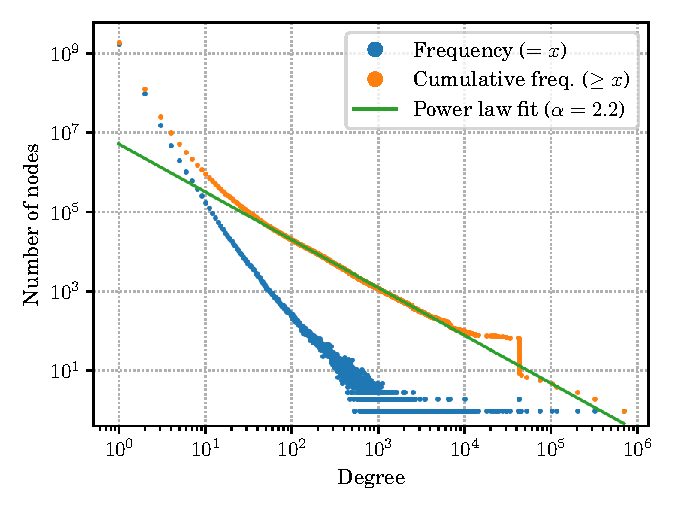
\includegraphics[width=\linewidth]{img/topology/inout/rev_in}
        \caption{In-degrees (``fork-degrees'')}
        \label{fig:inout_in_rev}
    \end{subfigure}\hfill%
    \begin{subfigure}{.49\textwidth}
        \centering%
        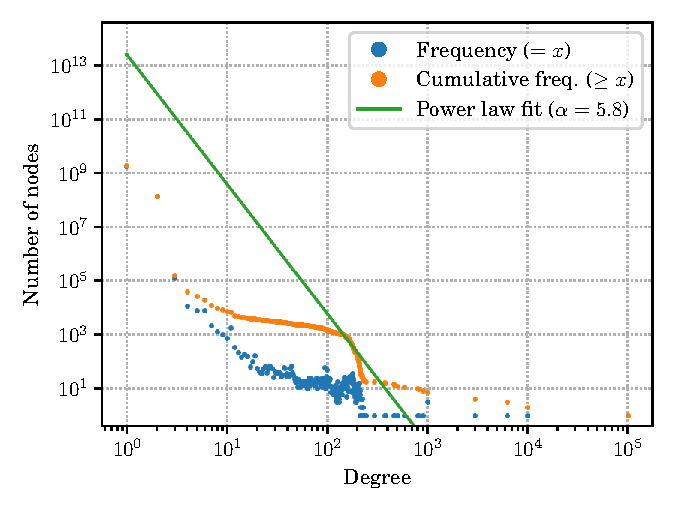
\includegraphics[width=\linewidth]{img/topology/inout/rev_out}
        \caption{Out-degrees (``merge-degrees'')}
        \label{fig:inout_out_rev}
    \end{subfigure}
    \caption{Degree distributions: Commit layer}
    \label{fig:inout_rev}
\end{figure}

The degree distributions for the commit layer are shown in
\cref{fig:inout_rev}.
As the parent/children terminology can be confusing when dealing with commits
(since \emph{parent commits} are \emph{children nodes} in the DAG), we
generally refer to the in-degree of commits as the ``fork-degree'', that is the
number of commits that were based on a specific commit, and to the out-degree as
the ``merge-degree'', the number of commits that were merged in a specific
commit.
The fork-degree distribution is very smooth with no notable threshold effect.
This can be explained by common development patterns: forks are generally
feature branches that are based on the latest revision in the main development
branch, which is generally random, so there is little reason to expect large
deviations from the naturally resulting power law.

The merge-degree distribution has a large gap after $d = 2$. The
vast majority of commits only have one parent, but occasionally two branches
are merged back together, which creates a merge commit with two parents. These
are the two most common cases, separated by one order of magnitude ($\approx
10^9$ simple commits, $\approx 10^8$ merge commits).
Commits with more than one parent are called ``octopus merges'', and are
exceedingly rare occurrences, generally not a part of standard development
workflows, which explains the gap of two orders of magnitude between $d = 2$
and $d = 3$. We expect most of these octopus merges with large degrees to be
generated by scripts in very peculiar environments, so the irregularities
observed in the tail of the distribution are not particularly surprising.
As the shape of this distribution is dominated by outliers and irregularities,
the power law fit is likely uninterpretable.

The outliers in these distributions are usually experiments aiming to generate
commits with inordinate amounts of parents. The largest degree in the out-degree
distributions is at $d = 10^6$, and comes from a GitHub repository called
\texttt{test-commit-many-parents-1m}, which contains two commits linked
together by one million of edges. It contains the most forked commit in the
archive.

\plotinout{rel+rev}{History layer}

\begin{figure}
    \centering
    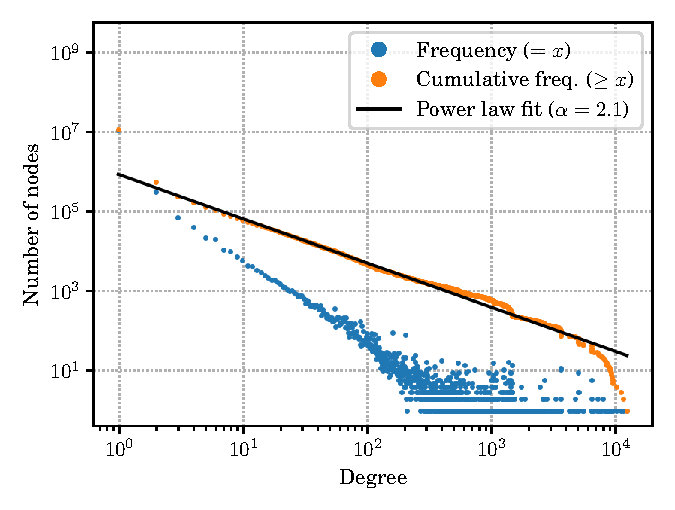
\includegraphics[width=.49\textwidth]{img/topology/inout/rev_in_rel}
    \caption{In-degrees of commits from releases}
    \label{fig:inout_rev_in_rel}
\end{figure}

The history layer's degree distribution, shown in \cref{fig:inout_rel+rev},
is extremely similar to the one of the commit layer as it is largely dominated
by the commits it contains. However, it is still interesting
to look at the in-degree distribution of the commit layer from the releases,
i.e., the distribution of the number of releases that point to a given commit.
It is shown in \cref{fig:inout_rev_in_rel}.  There is a noticeable threshold
effect between $d = 1$ and the rest of the distribution, again attributable to
development practices. Releases, or named tags, are generally used to denote
specific versions of a software. It makes little sense to have two different
versions pointing at a single commit, since there would be no code changes to
justify the version increment. Occasionally releases can be used to annotate
some specific milestones in a project in addition to its current version, so
commits pointed by more than two releases do have some significance, although
their importance diminishes rapidly in the distribution.

\plotinout{ori+snp}{Hosting layer}

The distribution of the hosting layer is shown in \cref{fig:inout_ori+snp}.
Since within the history layer of the graph, an origin cannot have ancestors
and a snapshot cannot have descendants, the two distributions show very
different things.
The out-degree distribution describes the number of snapshots associated to
each origin. This is not an intrinsic property of development workflows
because it is highly dependent on the crawling process of Software Heritage: if
a repository changes constantly but is only visited once every month, the
distribution will not capture how frequently the repository is updated, but
rather how often the crawler visits it.
On the other hand, the in-degree distribution describes the number of origins
associated to each snapshot, that is, the number of ``exact forks'' of a given
repository. This happens anytime time someone makes an exact copy of a
repository, for instance by clicking on the ``fork'' button in GitHub, without
then updating it with new commits or branches: a new origin is created, but it
points to the same repository state as the first origin.


% \begin{figure}%
% \subfigure{\includegraphics[width=6cm]{#1.png}}%
% \subfigure{\includegraphics[width=6cm]{#1_ehat.png}}%
% \subfigure{\includegraphics[width=6cm]{#1_fit.png}}%
% \end{figure}%
% 
% \plotdistribs{img/topology/inout/full_in}
% \plotdistribs{img/topology/inout/full_out}
% \plotdistribs{img/topology/inout/dir+cnt_in}
% \plotdistribs{img/topology/inout/dir+cnt_out}
% \plotdistribs{img/topology/inout/rev_in}
% \plotdistribs{img/topology/inout/rev_out}
% \plotdistribs{img/topology/inout/rel+rev_in}
% \plotdistribs{img/topology/inout/rel+rev_out}
% \plotdistribs{img/topology/inout/ori+snp_in}
% \plotdistribs{img/topology/inout/ori+snp_out}

% Breakdown for each type, not needed according to the protocol
% \begin{figure}[h]
% \subfigure{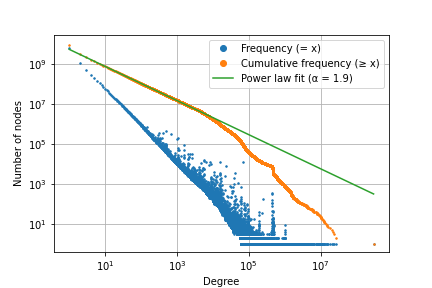
\includegraphics[width=6cm]{img/topology/inout/cnt_in_dir.png}}
% \subfigure{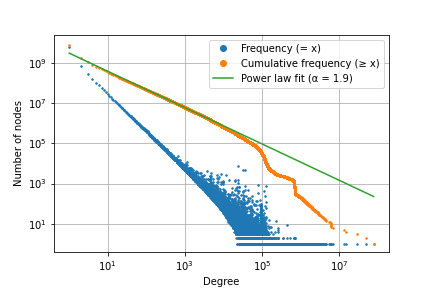
\includegraphics[width=6cm]{img/topology/inout/dir_in_all.png}}
% \subfigure{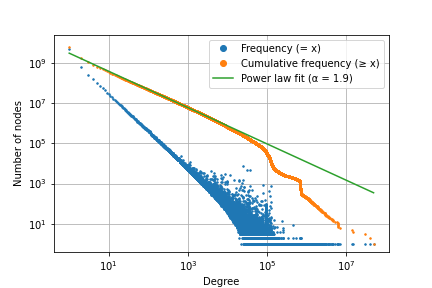
\includegraphics[width=6cm]{img/topology/inout/dir_in_dir.png}}
% \subfigure{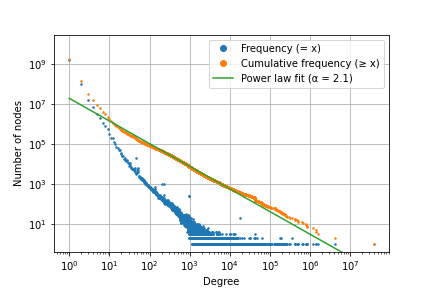
\includegraphics[width=6cm]{img/topology/inout/dir_in_rev.png}}
% \subfigure{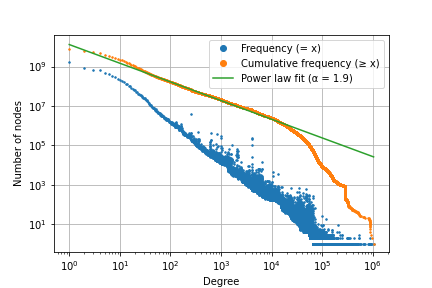
\includegraphics[width=6cm]{img/topology/inout/dir_out_all.png}}
% \subfigure{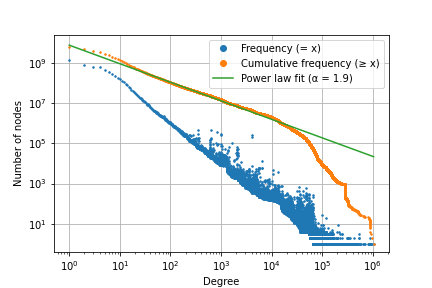
\includegraphics[width=6cm]{img/topology/inout/dir_out_cnt.png}}
% \subfigure{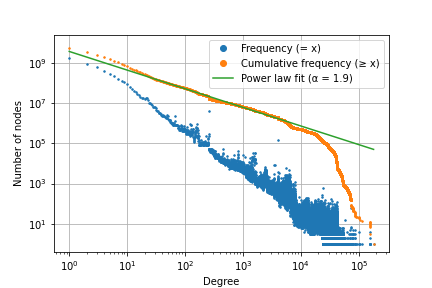
\includegraphics[width=6cm]{img/topology/inout/dir_out_dir.png}}
% \subfigure{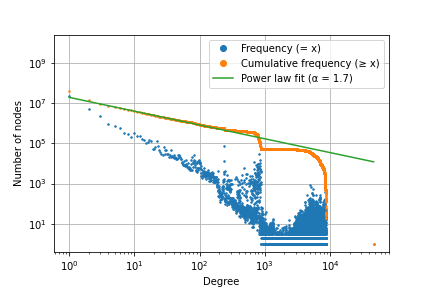
\includegraphics[width=6cm]{img/topology/inout/dir_out_rev.png}}
% \subfigure{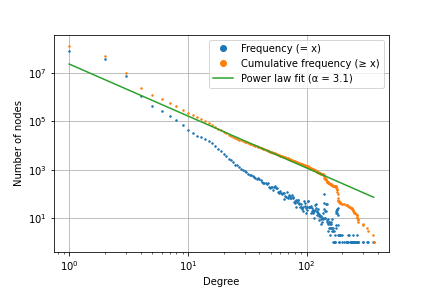
\includegraphics[width=6cm]{img/topology/inout/ori_out_snp.png}}
% \subfigure{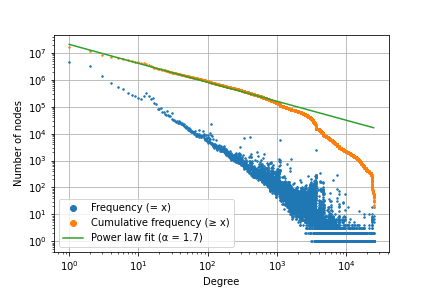
\includegraphics[width=6cm]{img/topology/inout/rel_in_snp.png}}
% \subfigure{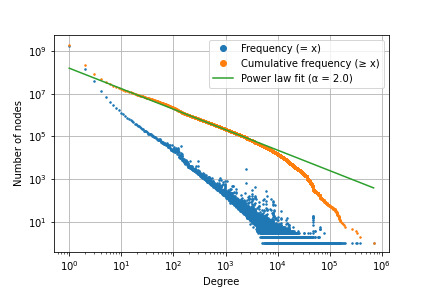
\includegraphics[width=6cm]{img/topology/inout/rev_in_all.png}}
% \subfigure{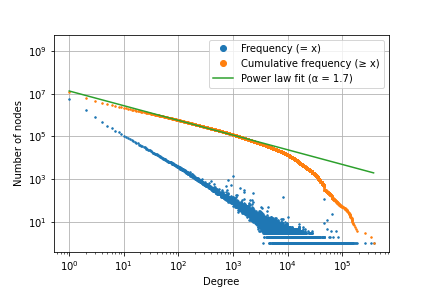
\includegraphics[width=6cm]{img/topology/inout/rev_in_dir.png}}
% \subfigure{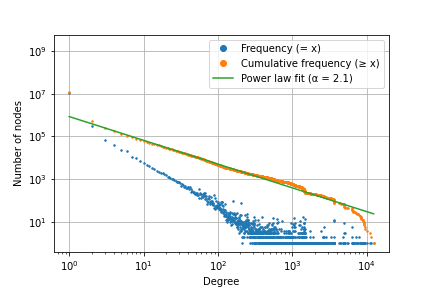
\includegraphics[width=6cm]{img/topology/inout/rev_in_rel.png}}
% \subfigure{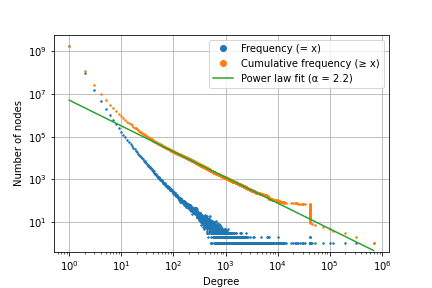
\includegraphics[width=6cm]{img/topology/inout/rev_in_rev.png}}
% \subfigure{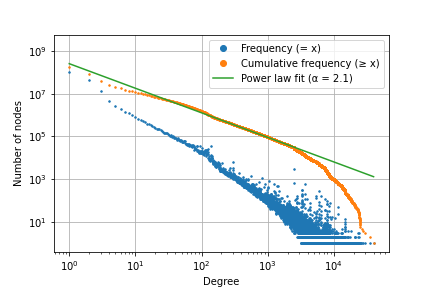
\includegraphics[width=6cm]{img/topology/inout/rev_in_snp.png}}
% \subfigure{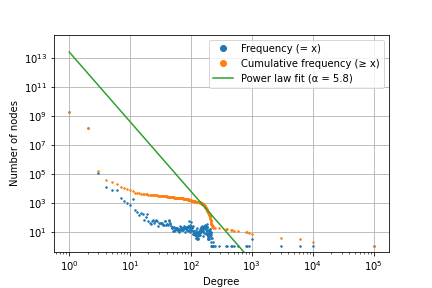
\includegraphics[width=6cm]{img/topology/inout/rev_out_rev.png}}
% \subfigure{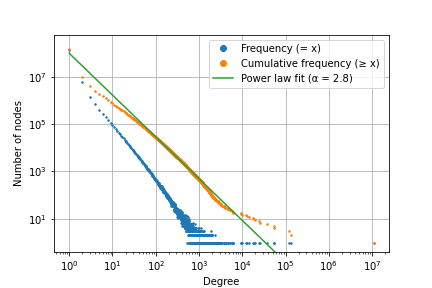
\includegraphics[width=6cm]{img/topology/inout/snp_in_ori.png}}
% \subfigure{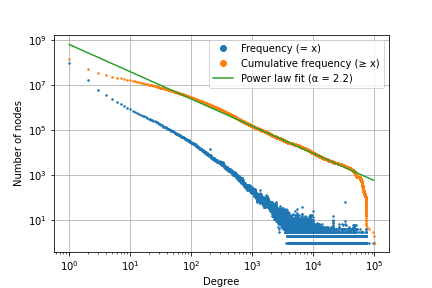
\includegraphics[width=6cm]{img/topology/inout/snp_out_all.png}}
% \subfigure{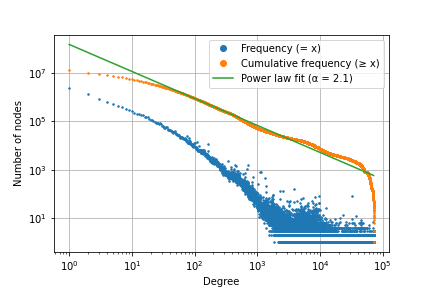
\includegraphics[width=6cm]{img/topology/inout/snp_out_rel.png}}
% \subfigure{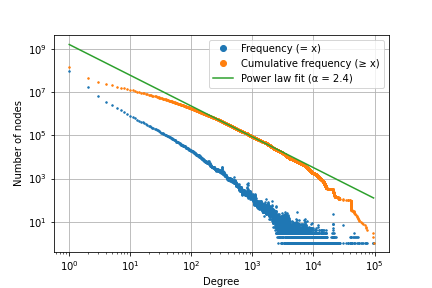
\includegraphics[width=6cm]{img/topology/inout/snp_out_rev.png}}
% \end{figure}
% 
\subsection{Local undirected clustering distribution}

\begin{figure}
    \begin{subfigure}{.49\textwidth}
        \centering
        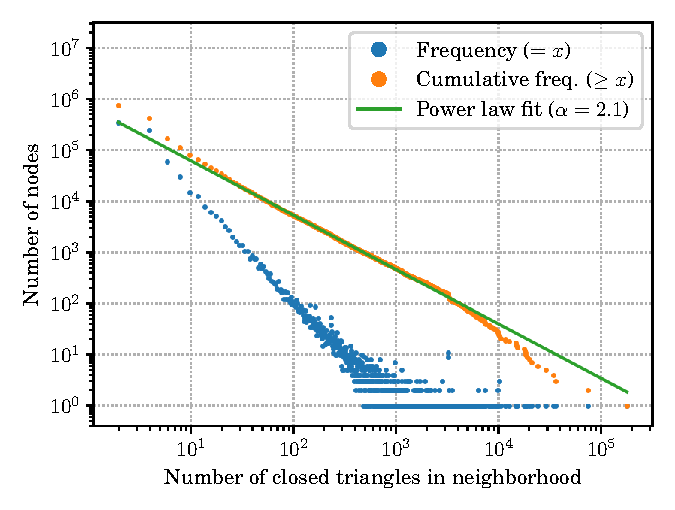
\includegraphics[width=\linewidth]{img/topology/clusteringcoeff/full}
        \caption{Full graph}
        \label{fig:clustering_full}
    \end{subfigure}\hfill
    \begin{subfigure}{.49\textwidth}
        \centering
        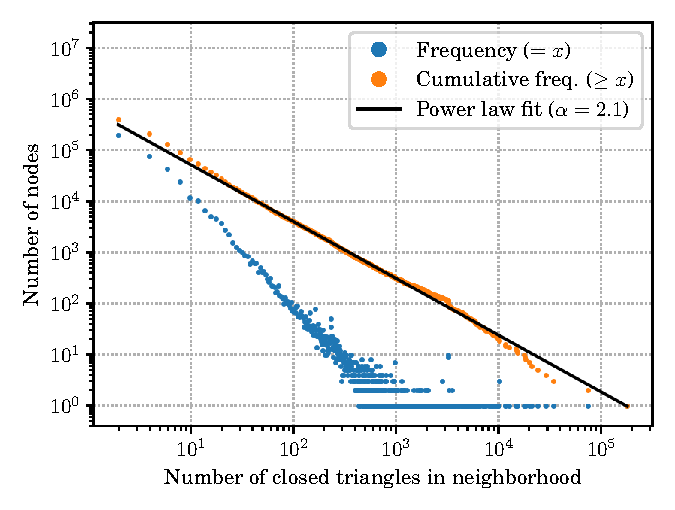
\includegraphics[width=\linewidth]{img/topology/clusteringcoeff/dir+cnt}
        \caption{Filesystem layer}
        \label{fig:clustering_dir+cnt}
    \end{subfigure}
    \newline
    \begin{subfigure}{.49\textwidth}
        \centering
        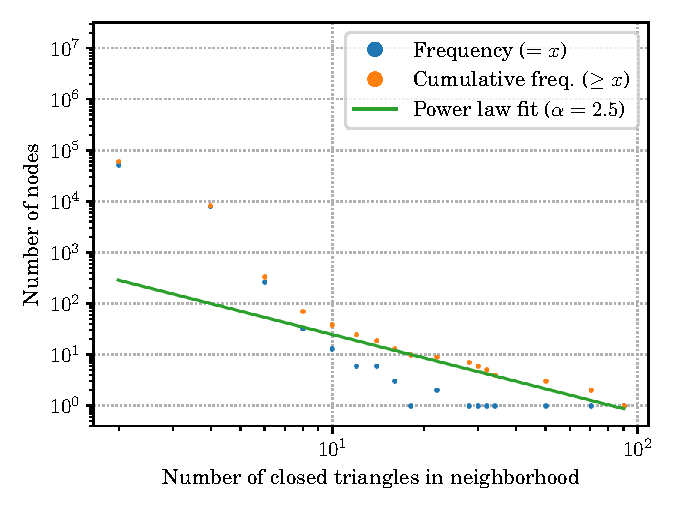
\includegraphics[width=\linewidth]{img/topology/clusteringcoeff/rev}
        \caption{Commit layer}
        \label{fig:clustering_rev}
    \end{subfigure}\hfill
    \begin{subfigure}{.49\textwidth}
        \centering
        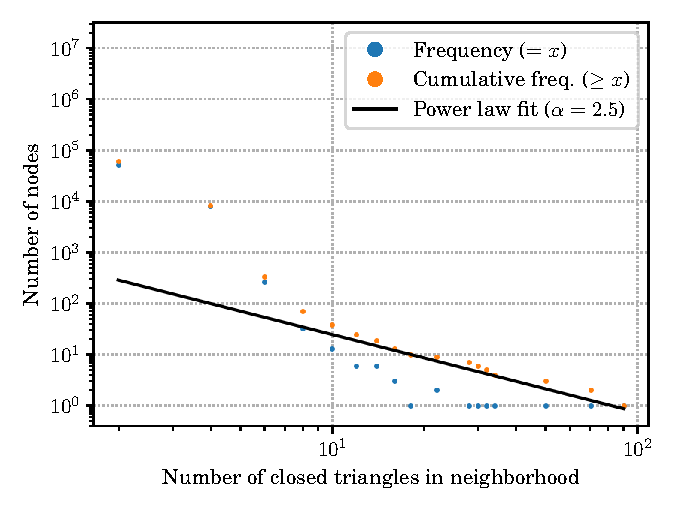
\includegraphics[width=\linewidth]{img/topology/clusteringcoeff/rel+rev}
        \caption{History layer}
        \label{fig:clustering_rel+rev}
    \end{subfigure}

    \caption{Clustering distributions (0.1\% uniform sample)}
    \label{fig:clustering}
\end{figure}%

We compute the local clustering distribution on the different layers of the
undirected graph, which describes the extent to which the nodes cluster
together in tight cliques. In a DAG this coefficient is always 0 since a
closed triangle corresponds to a cycle. However, the distribution of the number
of closed triangles in the undirected version of the graph, shown
in \cref{fig:clustering_full} can be interpreted meaningfully.

Again, the distribution for the full graph is completely dominated by the
filesystem layer and cannot be interpreted on its own; each layer has to be
looked at individually.
In the filesystem layer, a closed triangle corresponds to a file or a directory
being both in a directory $D$ and in a subdirectory $D'$ of $D$. A common
instance of this happening is when developers copy the contents of a directory
in a ``backup'' or ``old'' directory to take a snapshot of a previous version
of the directory.  \Cref{fig:clustering_dir+cnt} shows the frequency of these
triangles forming in the filesystem layer, with an apparent scale-invariant
regularity.

In the commit layer, the closed triangles correspond to a merge commit $C$ with
two parents $A$ and $B$, with $B$ being a parent of $A$. This often happens
when merging multiple commits using the ``no fast forward'' strategy
(\texttt{--no-ff} in Git). Here, the distribution (\cref{fig:clustering_rev})
displays a similar pattern to what we observed in the out-degree distribution
of the commit layer (\cref{fig:inout_out_rev}): the two common cases are
having one or two closed triangles, while having more triangles requires an
octopus merge and is relatively rare in most development workflows, which
explains the important threshold effect for $n > 2$.

Being a bipartite graph, the undirected hosting layer cannot contain closed
triangles and its local clustering distribution is therefore not represented
here.

% \plotdistribs{img/topology/clusteringcoeff/full}
% \plotdistribs{img/topology/clusteringcoeff/dir+cnt}
% \plotdistribs{img/topology/clusteringcoeff/rev}
% \plotdistribs{img/topology/clusteringcoeff/rel+rev}

\subsection{Connected components size distribution}

\begin{figure}
    \centering
    \begin{subfigure}{.49\textwidth}
        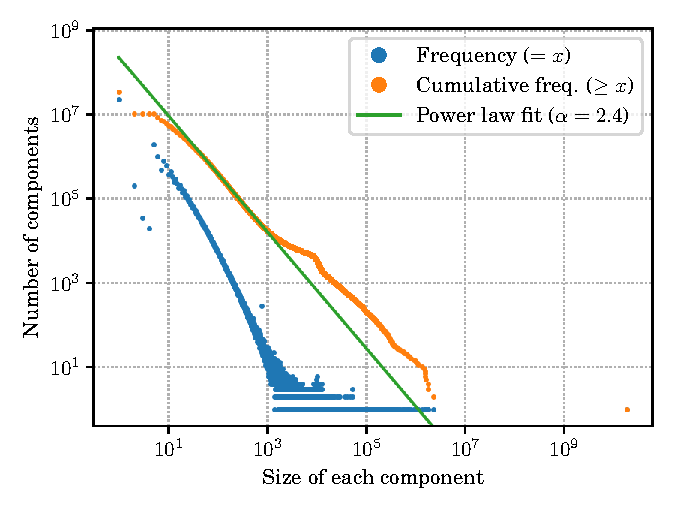
\includegraphics[width=\linewidth]{img/topology/connectedcomponents/full}
        \caption{Full graph}
        \label{fig:connectedcomponents_full}
    \end{subfigure}\hfill
    \begin{subfigure}{.49\textwidth}
        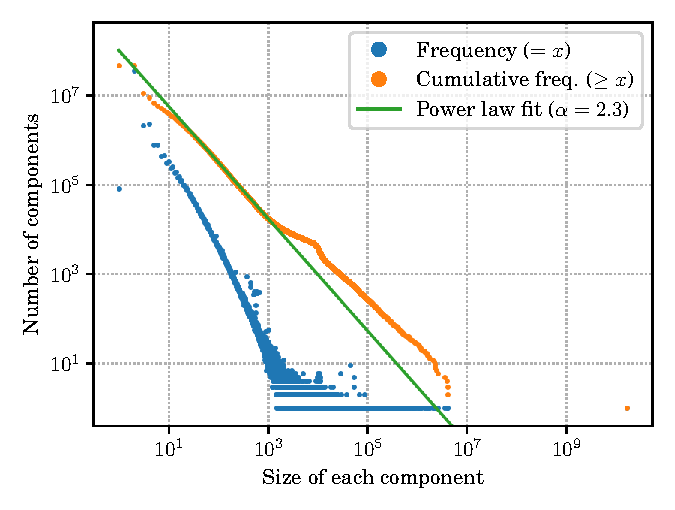
\includegraphics[width=\linewidth]{img/topology/connectedcomponents/dir+cnt}
        \caption{Filesystem layer}
        \label{fig:connectedcomponents_dir+cnt}
    \end{subfigure}
    \newline
    \begin{subfigure}{.49\textwidth}
        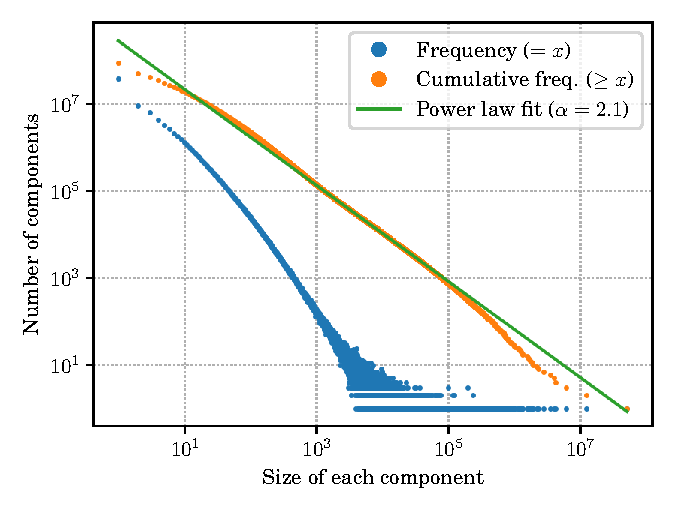
\includegraphics[width=\linewidth]{img/topology/connectedcomponents/rev}
        \caption{Commit layer}
        \label{fig:connectedcomponents_rev}
    \end{subfigure}\hfill
    \begin{subfigure}{.49\textwidth}
        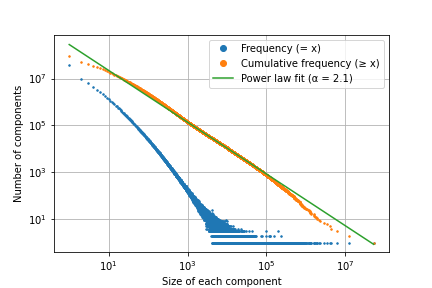
\includegraphics[width=\linewidth]{img/topology/connectedcomponents/rel+rev}
        \caption{History layer}
        \label{fig:connectedcomponents_rel+rev}
    \end{subfigure}
    \newline
    \begin{subfigure}{.49\textwidth}
        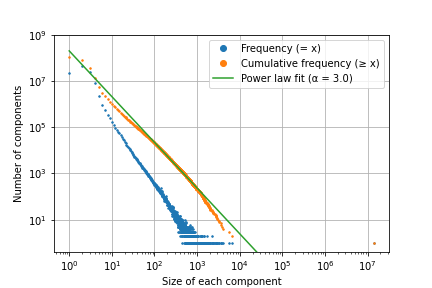
\includegraphics[width=\linewidth]{img/topology/connectedcomponents/ori+snp}
        \caption{Hosting layer}
        \label{fig:connectedcomponents_ori+snp}
    \end{subfigure}

    \caption{Connected components distributions}
    \label{fig:connectedcomponents}
\end{figure}

In this experiment, we symmetrize the graph to treat it as an undirected graph
and use a breadth-first traversal to compute the sizes of its weakly connected
components (WCC). \Cref{tab:wcc-stats} shows a breakdown of the number of
components and sizes of the largest components for each layer. In the entire
graph, we find a giant component of 18.9 billion nodes, in which a whole 97.8\%
of the nodes in the graph are reachable from one another by following
undirected edges. The size distribution for the full graph shown in
\cref{fig:connectedcomponents_full} clearly indicates the extent to which the
largest connected component is an outlier that dominates the entire
distribution, being 8345 times larger than the second largest.

\begin{table}
  \centering
  \caption{Connected components per layer}
  \label{tab:wcc-stats}
  \begin{tabular}[t]{l r r r}
      \textbf{Layer} & \textbf{\# of WCC}
                     & \textbf{Size of largest WCC}
                     & \textbf{\% of nodes in largest}
                     \\
    \hline
      Full graph       & \num{33104255}  & \num{18902683142} & 97.79\% \\
      Filesystem layer & \num{46286502}  & \num{16565521611} & 97.16\% \\
      Commit layer     & \num{88031649}  & \num{51543944}    & 2.61\% \\
      History layer    & \num{88040059}  & \num{52176239}    & 2.62\% \\
      Hosting layer    & \num{108342722} & \num{13841855}    & 4.82\%
  \end{tabular}
\end{table}


One could wonder whether this high connectivity results from a few
highly-connected nodes, like the empty file which is present in millions of
repositories.  Surprisingly, this turns out not to be the case: repeating the
same WCC experiment after removing the top 1 million of nodes with the largest
in-degrees from the graph still yields a giant component of about the same order
of magnitude (only about 5\% smaller). This implies that the connectivity of
the graph is resilient and does not depend on the existence of a few
high-degree nodes, and that those highly reused software artifacts exist in a
graph that is already well connected without them.
This finding is similar to what has been shown for the graph of the Web, where
removing pages which are central hubs and have a high PageRank does not
significantly reduces the connectivity of the graph.\cite{broder2000graph}

These observations apply similarly to the filesystem layer which again
dominates the distribution of the full graph. However, the distributions of the
commit and history layers shown in
\cref{fig:connectedcomponents_rev} and \cref{fig:connectedcomponents_rel+rev}
exhibit a very different graph connectivity. The largest component encompasses
less than 3\% of the graph, which indicates that the history layer can be
separated in reasonably sized units.
Furthermore, an in-depth investigation of this large component reveals that
most of the commits it contains belong to various forks of the Linux kernel,
which is suspected to be the largest open source software by number of commits
across all its different forks. We can infer from this observation that the
connected components of the history layer delineate structures of ``fork
networks'' in the graph, by clustering together projects that have a shared
development history.

The largest component in the hosting layer contains a relatively small share of
the layer's nodes (around 3\%), however it is still a relative outlier
containing 2051 times more nodes than the second-largest component. The larger
components generally contain repositories that are forked a lot, for example
the GitHub repository \texttt{jtleek/datasharing} which has been forked more
than 230 thousand times.  Even so, these outlier repositories do not explain
the existence of a component with more than seven million nodes, which is an
order of magnitude higher than the most forked repository. By walking random
paths in this component, it is possible to see some patterns that could explain
the size of this component.  One appears to be that beginners sometimes fork
well known repositories then rewrite their history to replace them with a
completely different content.  Every time this happens, it links together
completely unrelated networks of forks, which all aggregate in this large
component.

% \plotdistribs{img/topology/connectedcomponents/full}
% \plotdistribs{img/topology/connectedcomponents/dir+cnt}
% \plotdistribs{img/topology/connectedcomponents/rev}
% \plotdistribs{img/topology/connectedcomponents/rel+rev}
% \plotdistribs{img/topology/connectedcomponents/ori+snp}

\begin{comment}
\begin{figure}
    \centering
    \begin{subfigure}{.49\textwidth}
        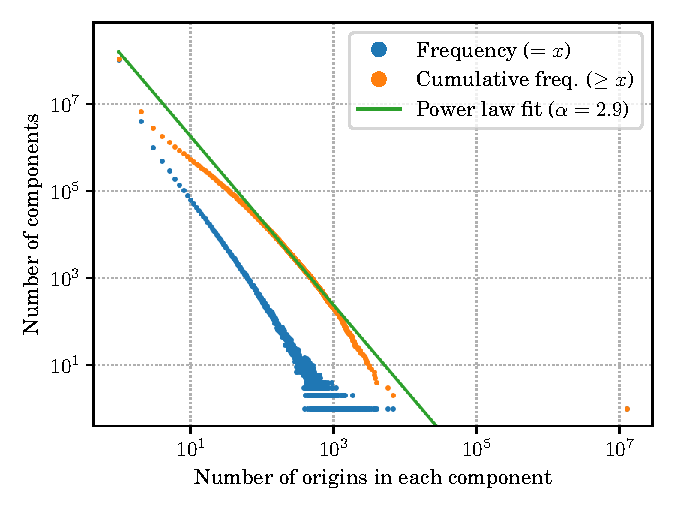
\includegraphics[width=\linewidth]{img/topology/connectedcomponents/by_origins/ori+snp}
        \caption{Hosting layer only}
        \label{fig:connectedcomponents_byorigins_ori+snp}
    \end{subfigure}
    \begin{subfigure}{.49\textwidth}
        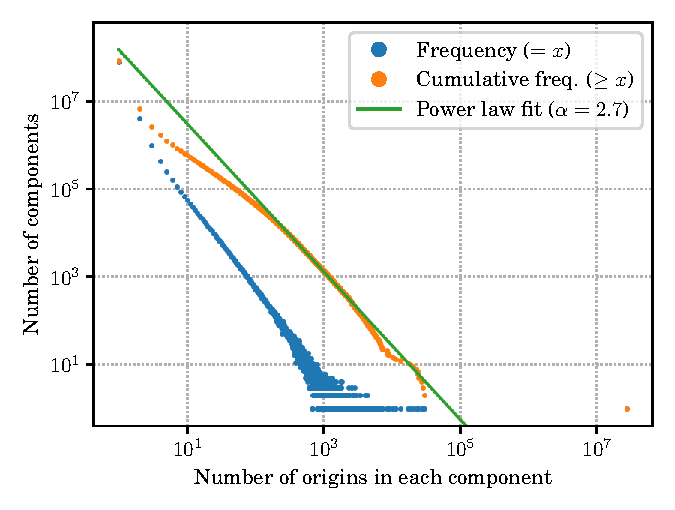
\includegraphics[width=\linewidth]{img/topology/connectedcomponents/by_origins/ori+snp+rel+rev}
        \caption{Hosting and history layers only}
        \label{fig:connectedcomponents_byorigins_ori+snp+rel+rev}
    \end{subfigure}
    \newline
    \begin{subfigure}{.49\textwidth}
        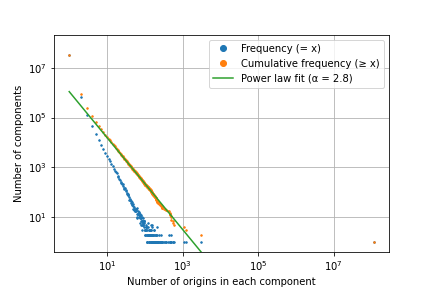
\includegraphics[width=\linewidth]{img/topology/connectedcomponents/by_origins/full}
        \caption{Full graph}
        \label{fig:connectedcomponents_full}
    \end{subfigure}\hfill

    \caption{Connected components size distributions by number of \emph{origins} in
    each component.}
    \label{fig:connectedcomponents_byorigins}
\end{figure}

% Integrate in prose ? discuss (or not) CC / layer. size= number of origin
% nodes

\begin{figure}
    \centering
    \begin{subfigure}{.49\textwidth}
        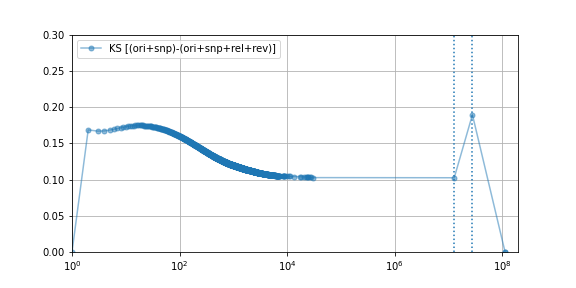
\includegraphics[width=\linewidth]{img/topology/connectedcomponents/by_origins/CC_KS_ori+snp_ori+snp+rel+rev.png}
        \caption{Hosting vs Hosting+History layers}
        \label{fig:KS_ori+snp+rel+rev}
    \end{subfigure}
    \begin{subfigure}{.49\textwidth}
        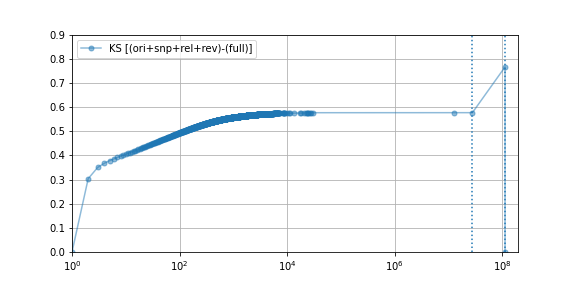
\includegraphics[width=\linewidth]{img/topology/connectedcomponents/by_origins/CC_KS_ori+snp+rel+rev_full.png}
        \caption{Hosting+History layer vs full graph.}
        \label{fig:KS_all}
    \end{subfigure}
    \caption{Kolmogorov-Smirnov distance between weighted connected component size distribution functions.}
    \label{fig:KS}
\end{figure}


The histograms of the sizes of the connected components per layer are completed
by comparing these distributions while merging some layers.  We display the
three distributions of their sizes expressed as a function of the number of
nodes of type origin only \cref{fig:connectedcomponents_byorigins}, and their
differences using the Komogorov-Smirnov distance \cref{fig:KS}.

The first point of interest concerns the gap for s=2, which corresponds to the
$\%$ of isolated origins (i.e., a single origin per connected component) which
are found in components containing several origins if we integrate the
following layer.

Out of a total of 147 million origins, $71.6\%$ are isolated origins in
separate connected components within the Hosting layer. This number decreases
by $17\%$ when merging this layer with the History layer
(\cref{fig:KS_ori+snp+rel+rev}), and by $30\%$ when taking into account the
complete graph (\cref{fig:KS_all}).  The sharp negative variations at the
extreme right of these figures, correspond to the number of origins that
compose the giant cluster of the initial layer, plus the number of origins that
integrate the giant cluster when the next layer is taken into account
(respectively $10.2\%+8.8\%=18.9\%$, and $57.8\%+18.9\%=76.8\%$)

This allows us to conclude that the growth of the giant component does not
occur only by aggregation of connected components containing isolated origins.
This is further confirmed by the progressive decrease of the curve at
intermediate sizes (left figure), which indicates that the components of these
sizes include more origins, previously included in components of smaller sizes.

This aggregation phenomenon concerns all layers and all sizes of components,
limiting the usefulness of partitioning the graph on the basis of these two
criterion alone.
\end{comment}


\subsection{Shortest path lengths}

% \plotdistribs{img/topology/avgpath/dir+cnt}
% \plotdistribs{img/topology/avgpath/rev}

\begin{figure}
    \centering
    \begin{subfigure}{.49\textwidth}
        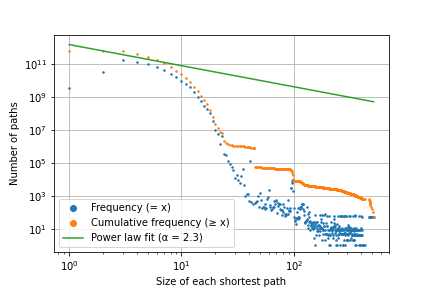
\includegraphics[width=\linewidth]{img/topology/avgpath/dir+cnt}
        \caption{Filesystem layer (10\% uniform sample)}
        \label{fig:avgpath_dir+cnt}
    \end{subfigure}\hfill
    \begin{subfigure}{.49\textwidth}
        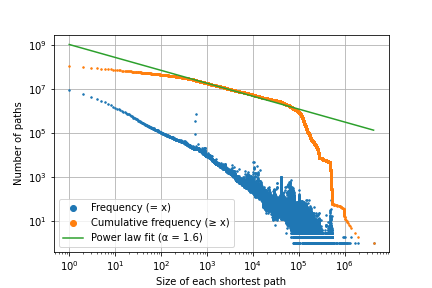
\includegraphics[width=\linewidth]{img/topology/avgpath/rev}
        \caption{Commit layer}
        \label{fig:avgpath_rev}
    \end{subfigure}
    \caption{Shortest path length distributions}
    \label{fig:avgpath}
\end{figure}

The last topological property we look at is the average length of the shortest
paths between root and leave nodes in the filesystem
(\cref{fig:avgpath_dir+cnt}) and commit layer (\cref{fig:avgpath_rev}), as
defined in \cref{sec:metho:avgpath}.
These have directly transposable meanings in software development. In the
filesystem layer, they correspond to the minimum directory depth at which a
given blob can be found on average. In the commit layer, they are the lengths
of the commit chains from the first commit of the project to the heads of the
branches.  These are particularly interesting alongside the degree
distributions, as they help us understand the shape of the graph given its
density.

We saw in \cref{sec:topo:degrees} that the filesystem layer was dense,
with nodes in close proximity with each other.  The distribution obtained in
\cref{fig:avgpath_dir+cnt} gives an idea of the depth of the files in the
directory trees, which interestingly appear in a very characteristic
configuration. The distribution does not exhibit scale-invariant behavior,
suggesting that its mean does not diverge.  Typically, most files seem to be at
a depth of less than around 15, with the frequency of deeper files dropping
sharply after that threshold.  The most common depth is 3, and files less than
4 directory deep are less common than files at a depth between 4 and 8. This
makes some intuitive sense, as the source files which are modified pretty often
are generally organized inside directory hierarchies, and rarely at the top
level.

In contrast, \cref{sec:topo:degrees} showed that the history layer was
sparse with an average degree close to one, indicating that it was mainly
constituted of degenerate strings of commits. \Cref{fig:avgpath_rev} shows us
the distribution of the lengths of these strings, which appears to have some
scale invariance. Because these lengths can be interpreted as the ``age'' of a
given project measured in number of commits, it makes sense that they would
follow a normal distribution with infinite variance.
A few outliers are also present in the tail of the distribution, mostly test
projects like the GitHub repository \texttt{cirosantilli/test-many-commits-1m}
which contains two million commits.

\section{Discussion}
\label{sec:topology-discussion}

Our results shed light on some properties of the software development graph
which have important implications for empirical research and large scale
analysis.

The first salient characteristic is the large topological disparity between the
different layers that constitute the graph, both at the local level and in
their global structure. If we break down the graph in three layers, we see that
they have dramatically different shapes, densities and connectivities.

The filesystem layer contains 90\% of the nodes and 97\% of the edges of the
full graph, and thus largely dominates its high-level topological properties.
This layer is dense and highly connected, due to the high amounts of
deduplication of the software artifacts it contains. This high connectivity
naturally leads to the existence of a giant connected component, containing
more than 97\% of all the files and directories in the graph that are all
reachable from each other by simply following directory hierarchy vertices.
The degree distributions in the layer have a heavy tail, with a very high
frequency of nodes exceeding the average degree.
The directory trees have a characteristic depth with a converging average, with
only a few outliers with a hierarchy depth larger than around 20 nested
directories.

\begin{comment}
\begin{figure}
\begin{center}
  \includegraphics[width=0.6\textwidth]{lol.png}
\end{center}
\caption{Distributions with heavy tails/high kurtosis do not have a converging
average: commit chains do not have a characteristic length (high kurtosis) but
do have a typical average degree (low kurtosis); directories do not have a
typical average degree but do have a characteristic depth.}
\end{figure}
\end{comment}

In contrast, the history layer has virtually the exact opposite topological
properties. It is sparse and mildly connected, mainly constituted of almost
degenerate chains of commits, with relatively low deduplication compared to the
filesystem layer. Its largest component is less than 3\% the size of the entire
graph, which implies that the nodes are well separated within the layer.
Commits have a characteristic out-degree, with very few outliers that merge
more than 3 commits together. However, the commit chains do not have a bounded
height, and the distribution of the shortest path lengths between the root
commits and the branch heads has a heavy tail, with a high frequency of chains
longer than the average height.

Finally, the hosting layer is a bipartite graph containing a small fraction of
the nodes in the graph. It is also sparse and minimally connected, with some
deduplication for identical forks, which are a frequent occurrence in modern
hosting platforms.

An important practical implication of these findings is that because the
filesystem vertices largely aggregate in a giant component, it is not possible
to apply strict component separation to partition the entire graph in smaller
tightly connected clusters in order to perform scale-out computations. The
filesystem layer should be seen as a dense network of highly connected software
artifacts, and there is no obvious way to remove high-connectivity nodes to
break it down into multiple disconnected subgroups.  However, because the
hosting and history layers are sparse, have a low connectivity and smaller
giant components, it is possible to easily separate them into multiple
partitions that can be processed in parallel while retaining the performance
advantages of exploiting node locality within them.

Another key point relevant for empirical software engineering studies is that
the distributions studied in this article often have heavy tails and a
generally high kurtosis (i.e., a high propensity to produce outliers). This
implies that there is often no obvious rule to filter out outliers after a
given threshold, as they are an integral part of the distributions' nature.  As
such, empirical studies should be cautious to systematically justify how they
filter outliers in their methodology, and consider sampling biases as potential
threats to validity.

\section{Threats to validity}%
\label{sec:topology-threats}

\subsection{Internal validity}

This study closely follows the registered protocol described
in~\cite{msr-2020-topology}, and extracts the quantitative data required to
answer its three research questions from the Software Heritage graph dataset.
This data is extracted and analyzed using the algorithms and statistical tools
described in the protocol, without any particular changes to the methodology.
However, while writing the protocol, we underestimated the execution time of
two algorithms, which we were not able to run on the entire graph.

According to our estimates, the path length distribution of the filesystem
layer would have taken around two months to compute on an expensive machine,
thus we restricted ourselves to a subsample of 10\% of the nodes in the
filesystem layer. However, we were able to run this algorithm on the entire
commit layer in around 3 hours, without resorting to subsampling.

More importantly, we drastically underestimated the time required to compute
the clustering coefficient of the entire undirected graph, which would have
taken several years on our hardware. We had to analyze a subsample of
0.1\% of the entire graph, which is in line with the sample sizes of
clustering coefficient estimates in other analyzes of large
networks.

As this study is exploratory in nature, we anticipated the possibility of
having to resort to sampling in the
protocol~\cite[Section 7]{msr-2020-topology}.

One last potential internal threat is the validity of the dataset itself.
Because this study is the first of its kind ever performed on the graph of
software development, there is no existing dataset to which its properties can
be cross-compared. We performed a series of manual robustness checks to ensure
that the properties were consistent to our own expectations, which allowed us
to iteratively find and correct errors in our dataset building pipeline.
However, there is no way to guarantee that these checks were exhaustive.

\subsection{External validity}

While our data corpus is the largest dataset of software development history,
and \emph{aims} to be as exhaustive as materially possible, it remains a
subsample of the entirety of public software commons, and as such the way it is
constructed is a source of various potential bias.

\paragraph{Exhaustiveness of VCS and package managers.}
Software Heritage covers the most popular DVCS (Git, Mercurial, SVN…) as well
as distribution and language-specific packages (dpkg, Nix, Python, NodeJS…),
and regularly adds support for new systems. The dataset does not cover all the
less commonly used systems (Bazaar, Darcs, CVS, …). If software development
patterns on these platforms are significantly different, this study cannot
properly capture them in a representative manner.

\paragraph{Exhaustiveness of data sources.}
Likewise, the representativeness of the study is limited by the extent of the
data source coverage of Software Heritage. The archive contains the main
centralized software forges and package repositories (GitHub, Gitlab,
Bitbucket, PyPI, Debian, NixOS, …), as well as instances of decentralized
forges (e.g., various self-hosted Gitlab or Phabricator instances). As the
archive cannot realistically cover the long tail of smaller self-hosted forges,
this is another source of popularity bias in the input dataset.

\paragraph{Archival process.}
The process of listing data sources and loading repositories and software
packages in the Software Heritage archive is heterogeneous across data sources,
which can skew the representativeness of the data. Data sources are crawled
at varying frequencies depending on multiple factors: for instance, some forges
support subscription-based APIs that allow the listers to crawl repositories as
soon as a change is pushed to them. Some repositories are considered more
critical to software infrastructures and are crawled daily. Other scheduling
heuristics are in place to maximize resource usage efficiency of data crawlers.
Overall, this means that the topology of the `hosting'' layer is endogenous to
the archival process, rather than being an intrinsic property of software
development. This is mainly reflected in the number of snapshots that neighbor
a given origin, since more frequent crawling generally produces more snapshots.

\paragraph{Non-software data.}
We acknowledge the habit of developers to use software development platforms
and hosts for non-software projects (e.g., collaborative writing, websites,
open datasets, art assets, etc.). However, we expect software development to be
the dominant content hosted in these platforms. We also assume that the results
of this work would be most useful for researchers when applied to similar
corpuses, which would contain the same kind of non-software data, as opposed to
carefully curated ones.
